\documentclass[prl,twocolumn,floatfix]{revtex4-2}

\usepackage{graphicx}
\usepackage{bm}

\usepackage{amsmath}
\usepackage{units}

\usepackage{hyperref}
\hypersetup{colorlinks=true, citecolor=blue, urlcolor=blue, linkcolor=blue}

\usepackage{todonotes}

\renewcommand{\vec}[1]{\boldsymbol{#1}}

\begin{document}
\title{Magnetic dichroism in darkfield UV photoemission electron microscopy}
\author{Maximilian Paleschke$^{1}$, David Huber$^{1}$, Cheng-Tien Chiang$^2$, Frank O. Schumann$^3$, Jürgen Henk$^1$, Wolf Widdra$^1$}

\affiliation{$^1$Institute of Physics, Martin Luther University Halle-Wittenberg, D-06099 Halle (Saale), Germany}

\affiliation{$^2$Institute of Atomic and Molecular Sciences, Academia Sinica, Taipei, Taiwan}

\affiliation{$^3$Max-Planck-Institut f\"{u}r Mikrostrukturphysik, 06120 Halle, Germany}

\email{wolf.widdra@physik.uni-halle.de}

\date{\today}

\begin{abstract}
    Photoemission electron microscopy (PEEM) has evolved into an indispensable tool for structural and magnetic characterization of surfaces at the nanometer scale. Particularly, synchrotron-radiation-based X-ray PEEM has emerged as a leading method for probing element-specific magnetic properties via magnetic circular dichroism (MCD) in core level photoemission. In laboratory settings, UV radiation is utilized for near-threshold PEEM, which, when combined with femtosecond lasers, offers the potential for ultrafast time resolution. However, the characterization of magnetic properties, such as local magnetic domain structures, has seen limited application in UV-PEEM, with studies reporting only weak magnetic dichroism effects for in-plane magnetization. 
    In this letter, we introduce the concept of darkfield PEEM for MCD in threshold photoemission. This method enables efficient MCD imaging with a significantly enhanced MCD contrast—by an order of magnitude—for in-plane magnetization, as demonstrated for Fe(001). This advancement paves the way for MCD imaging on femtosecond timescales using modern lasers. Darkfield PEEM imaging employs an aperture for photoelectron momentum selection in the back focal plane of the electron imaging column before forming the real-space image. While the general momentum dependence of the MCD contrast will be explained through symmetry considerations, the experimental results for Fe(001) will be quantitatively compared with state-of-the-art full-relativistic photoemission calculations.
\end{abstract}

\pacs{}

\maketitle
% Paragraph headings may be deleted in the final version .
\paragraph{Introduction.} Ultrafast spin and magnetization dynamics are exciting and rapidly growing fields in condensed matter physics with promising implications for both future research and device applications. Ultrafast imaging of magnetic domains on the micrometer scale is well established based on all-optical methods, as e.g. Kerr microscopy. On the nanometer scale, however, electron microscopy is the method of choice due to electrons short de Broglie wavelength. 
For imaging magnetic domains the magnetic circular dichroism (MCD) contrast is used in photoelectron emission microscopy (PEEM). The intensity recorded for a particular domain changes with the helicity of the incident radiation, thereby producing magnetic contrast without the need for an explicit electron spin detection. By tuning the incident X-ray radiation to a magnetic core level absorption edge, substantial and element-specific MCD asymmetries have been reported. With the wide availability of tunable synchrotron radiation, this technique of XMCD-PEEM is well established for magnetic domain imaging on the nanometer scale and for slow dynamics. However, the pulse length of synchrotron radiation of typically 30-50 ps renders XMCD-PEEM unsuitable on ultrafast timescales. 
Replacing the incident X-ray radiation by ultrashort laser pulses solves this issue straightforwardly and allows for pump-probe experiments on a few femtoseconds timescale. In addition, experiments can be performed in the laboratory with UV laser sources. 
With UV light, electrons close to the Fermi level are excited to energies slightly above the escape threshold. However, the reported MCD contrasts are quit small in threshold photoemission, especially for in-plane magnetization. 

% Determined by the laser photon energy, photoelectrons are excited from the valence band to energies slightly above the escape threshold (i.e., a few tenths of an electronvolt above the vacuum level). Such concepts are not new and have been tested decades ago. 


In this letter we introduce the concept of darkfield PEEM for MCD in threshold photoemission. It allows efficient MCD imaging with an order-of-magnitude enhanced MCD contrast for in-plane magnetization as is demonstrated for Fe(001). It paves the way for MCD imaging on femtosecond timescales using modern lasers.
Darkfield PEEM imaging uses an aperture for photoelectron momentum selection in the back focal plane of the electron imaging column prior to forming the real space image. While the general momentum dependence of the MCD contrast will be rationalized by pure symmetry considerations, the experimental results for Fe(001) will be quantitatively compared with state-of-the-art full-relativistic photoemission calculations.

\todo[inline]{Review experiments}Respective experiments on Ni/Cu(001) with threshold PEEM revealed that the magnetic contrast is very small\todo[inline]{Give number} and therefore might not be sufficient for ultrafast imaging \todo[inline]{Add reference}.


\paragraph{Conceptual basis.} 

\begin{figure}
    \centering
    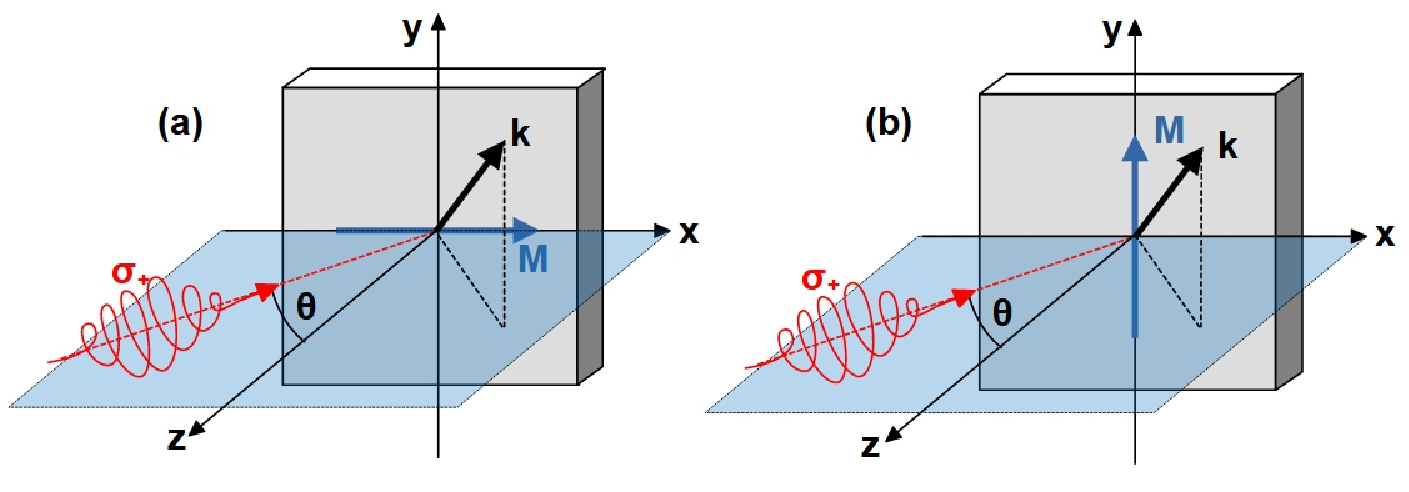
\includegraphics[width = \columnwidth]{symmetry}
    \caption{Symmetry analysis. A circular polarized laser pulse (orange, with helicity $\sigma_{+}$ impinges onto a magnetic domain (rectangular solid, with magnetization direction $\vec{M}$). The pulse's incidence direction and the surface normal ($z$-axis) span the scattering plane (blue; $xz$-plane). The off-normal detection of photoelectrons with wavevector $\vec{k}$ results in a chiral setup. If the scattering plane is a mirror plane of the lattice, the photoemission intensities for fixed $\vec{k}$ obey $I(\sigma_{+}, +\vec{M}) = I(\sigma_{-}, -\vec{M})$ (panel~a) or $I(\sigma_{+}, +\vec{M}) = I(\sigma_{-}, +\vec{M})$ (panel~b).}
    \label{fig:symmetry}
\end{figure}

For a conceptual approach we consider a surface with fourfold symmetry, as e.g. the (001) fcc or bcc surfaces with magnetic easy axes along the four [100] directions. Let's assume light incidence within one of the high-symmetry [100] direction as depicted in Fig.~\ref{fig:symmetry}. The photoemission intensity of electrons detected with off-normal wavevector $\vec{k}$ depends then on the helicity, $\sigma_{+}$ or $\sigma_{-}$, of the incident circular polarized laser radiation and on the two orientations $\pm M$ of the in-plane magnetization in a selected domain, yielding four intensities $I_{\vec{k}}(\sigma_{\pm}, \pm M)$ (shortened $I_{\pm \pm}$). The latter intensities are combined into the total intensity
\begin{align}
    I & \equiv I_{+ +} + I_{+ -} + I_{- +} + I_{- -}. 
\end{align}
In order to disentangle the two main contrast mechanisms we define appropriate asymmetries:
\begin{subequations}
\begin{align}
    A_{\mathrm{pol}} & \equiv \left[ \left( I_{+ +} + I_{+ -} \right) - \left( I_{- +} + I_{- -} \right) \right] / I,
    \label{eq:Apol}
    \\
    A_{\mathrm{ex}} & \equiv \left[ \left( I_{+ +} + I_{- -} \right) - \left( I_{+ -} + I_{- +} \right) \right] / I.
    \label{eq:Aex}
\end{align}    
\end{subequations}
In the polarization asymmetry $A_{\mathrm{pol}}$ the magnetization's orientation is averaged out; it thus encodes contrast due to the light's helicity (as if the domain were nonmagnetic). Contrast due to the exchange splitting is quantified by the exchange asymmetry $A_{\mathrm{ex}}$, in which one averages over the mutual orientations of helicity and magnetization. Note that the \textit{chiral geometry} for photoelectrons with \textit{off-normal} wavevector $\vec{k}$ results in magnetic dichroism and, hence, in magnetic contrast.

\paragraph{Experimental aspects.} Setup \ldots

The experimental results as well the conceptual ideas are supported by relativistic photoemission computations, briefly described in the Supplemental Material~\cite{Supplement}.

\paragraph{Contrast mechanisms.} In a first step we analyze the two main contrast mechanism: light polarization and exchange splitting.

The polarization asymmetry $A_{\mathrm{pol}}$, defined in Eq.~\eqref{eq:Apol} and depicted in Fig.~\ref{fig:Apol}, depends on the binding energy of the initial states. Both theoretical (top row) and experimental data (bottom row) show
that this contrast mechanism is sizable (with absolute values up to about $\unit[40]{\%}$ in theory and $\unit[20]{\%}$ in experiment) and thus cannot be ignored. 

\begin{figure*}
    \centering
    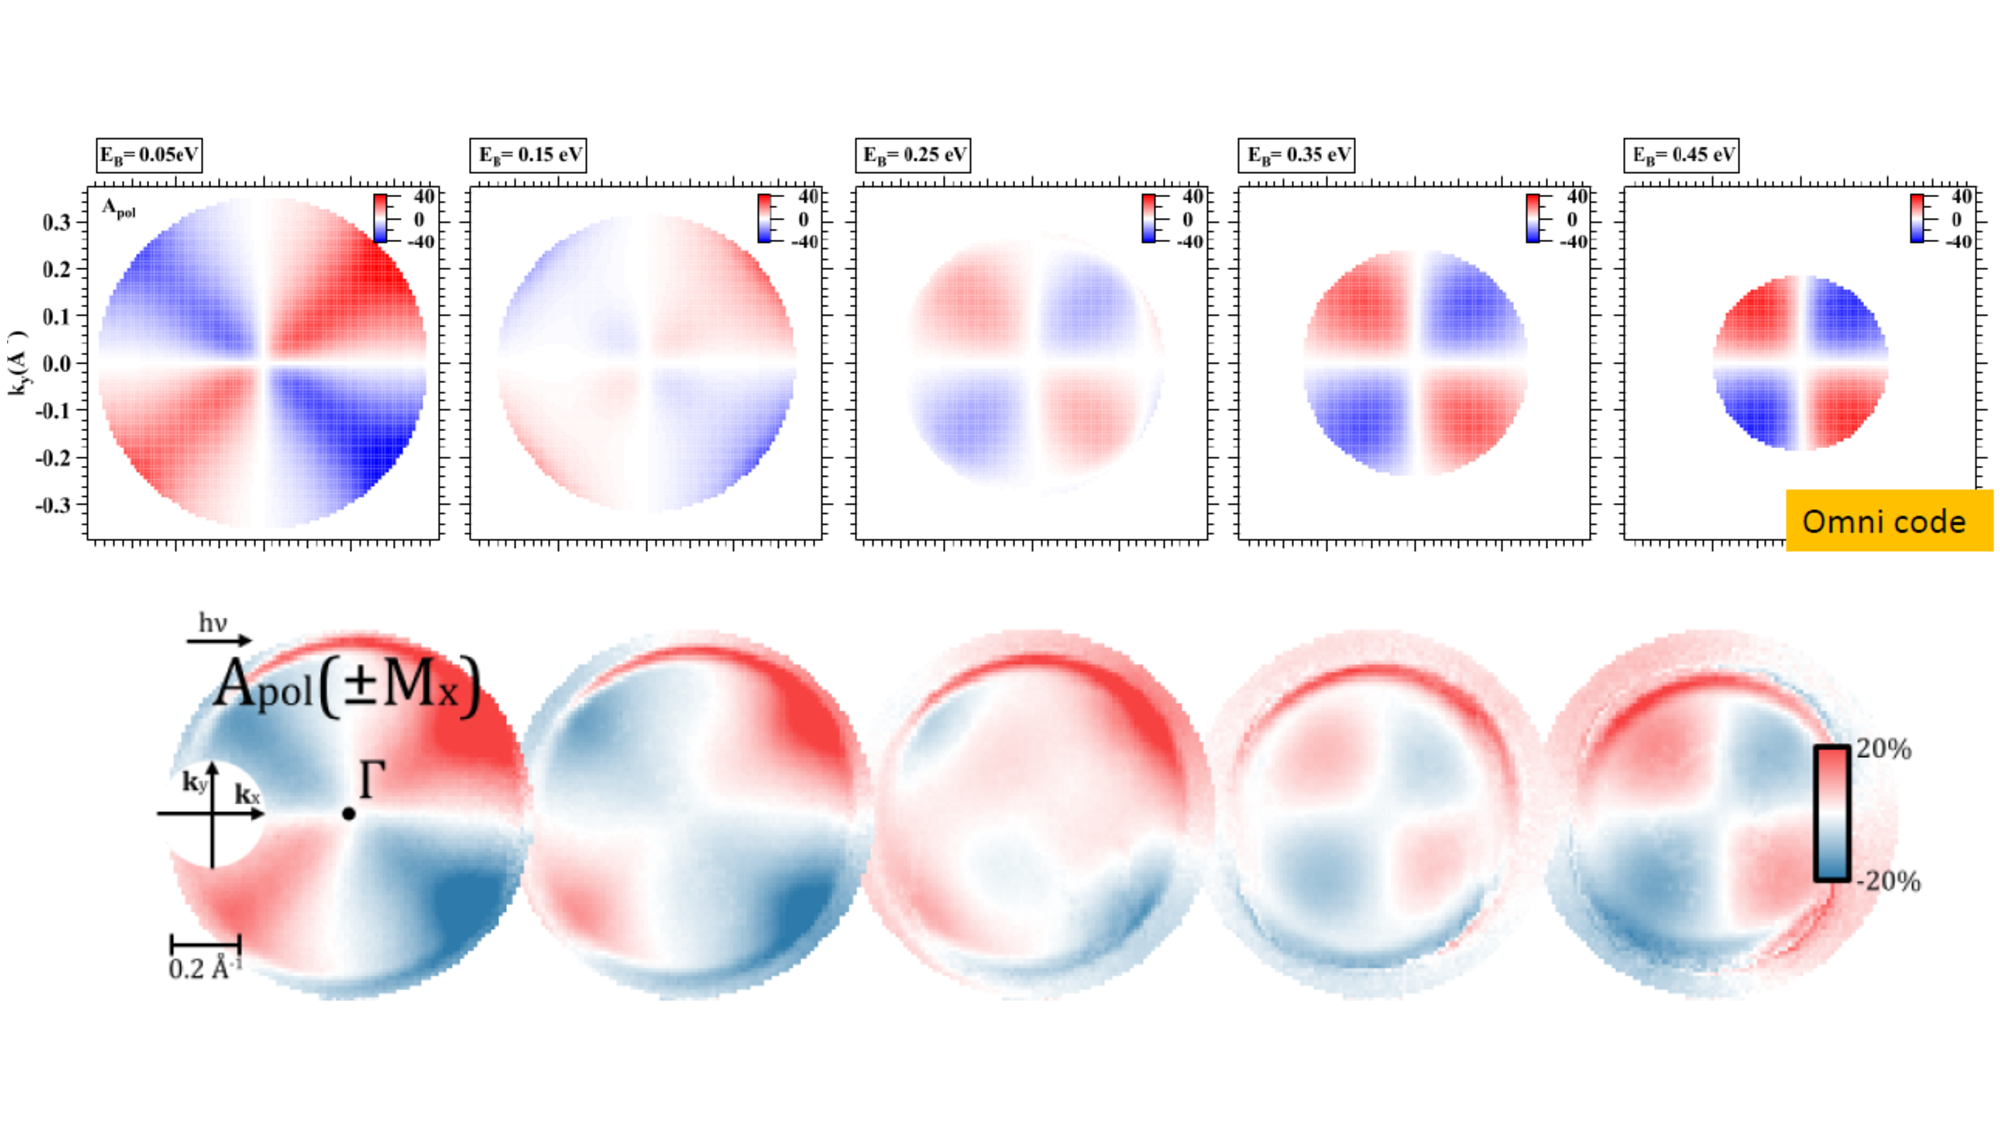
\includegraphics[width = 0.9\textwidth]{Apol}
    \caption{Polarization asymmetry $A_{\mathrm{pol}}$ of Fe(001) at selected binding energies versus wave vector $\vec{k}_{\parallel}$ of the photoelectrons. Top row: theoretical results obtained from photoemission calculations. The binding energy is indicated at each panel. The color scale, showing $A_{\mathrm{pol}}$ as defined in Eq.~\eqref{eq:Apol} in percent, is identical for all panels in this row. Bottom row: respective experimental results. The arrow marked $h \nu$ indicates the light incidence direction. $\Gamma$ is the center of the surface Brillouin zone ($\vec{k}_{\parallel} = $).}
    \label{fig:Apol}
\end{figure*}

The theoretical patterns (top row in Fig.~\ref{fig:Apol}) exhibit two nodal lines ($k_{x} = 0$ and $k_{y} = 0$). Moreover, one finds changes of sign if either $k_{x}$ or $k_{y}$ is reversed. These features are imposed by the symmetry of the setup. The experimental counterparts (bottom row) display the same features but slightly oblique or off-center, most clearly for binding energies with comparably small asymmetry (cf.\ $\unit[0.15]{eV}$ and $\unit[0.25]{eV}$). We attribute these deviations to imperfections in experiment, for example a small misalignment of the light incidence with respect to a crystal mirror plane and inhomogeneous magnetization in the surface layers. Moreover, we assume an electron self-energy that is independent of $k_{\parallel}$ (see \cite{Supplement}). Nevertheless, the agreement of experiment and theory shows that \ldots \todo{More here}

The energy-dependent exchange asymmetry $A_{\mathrm{ex}}$, defined in Eq.~\eqref{eq:Aex} and shown in Fig.~\ref{fig:Aex}, is smaller than $A_{\mathrm{pol}}$ (Fig.~\ref{fig:Apol}) (with absolute values up to $\unit[10]{\%}$ in theory and $\unit[6]{\%}$ in experiment). Nevertheless it exhibits a clear odd symmetry upon reversal of $k_{x}$; it does not change sign upon reversal of $k_{y}$, in contrast to $A_{\mathrm{pol}}$. Both features are dictated by the symmetry of the setup (see \cite{Supplement}).

\begin{figure*}
    \centering
    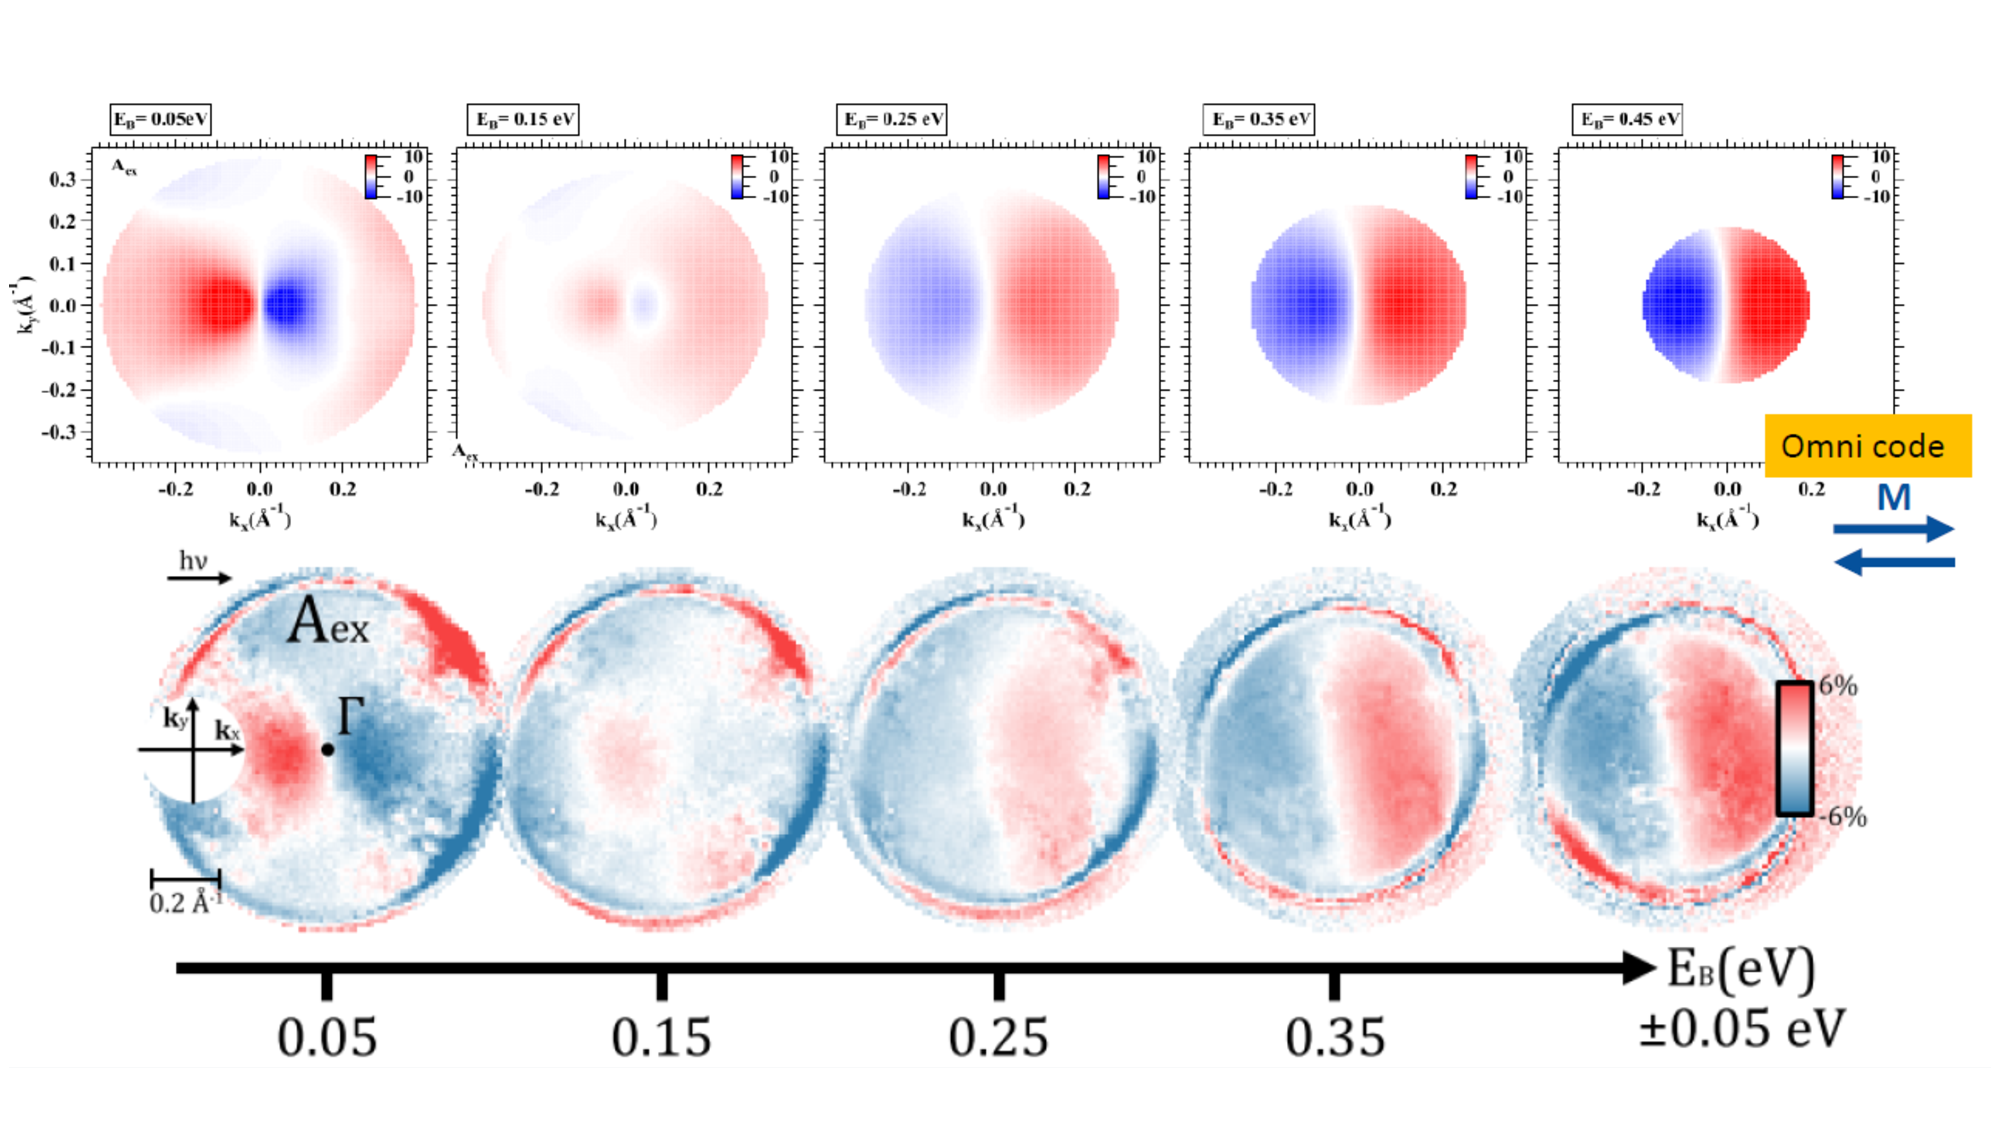
\includegraphics[width = 0.9\textwidth]{Aex}
    \caption{As Figure~\ref{fig:Apol}, but for the exchange asymmetry $A_{\mathrm{ex}}$ of Fe(001). The orientations of the magnetization are indicated by arrows on the right-hand side.}
    \label{fig:Aex}
\end{figure*}

The above findings support that the asymmetries $A_{\mathrm{pol}}$ and $A_{\mathrm{ex}}$ are suitable tools to disentangle and to quantify the main contrast mechanisms for domain imaging. 

\paragraph{Domain imaging.} Aperture, selection of wave vectors.

Center position of the aperture shows very weak contrast (Fig.~\ref{fig:Imaging}).

\begin{figure}
    \centering
    %\includegraphics{}
    \caption{Darkfield magnetic-circular dichroism imaging of Fe(100). Left: schematic, nine aperture positions \ldots. Right: domain imaging using the nine aperture positions.}
    \label{fig:Imaging}
\end{figure}

Sizable contrast in the other off-center positions of the aperture. Allows to image domain structure unequivocally. Size of contrast/asymmetry \ldots

\paragraph{Prospects.} The present investigation proves that magnetic domains can be imaged with a laser-equipped photoelectron emission microscope with high contrast using a momentum-selection of the detected photoelectrons. The common belief that a such PEEM provides only weak contrast is thereby refuted.

For a proof of principle we applied the proposed improvement to in-plane magnetized Fe(001) surfaces. However, the approach is general so that it can easily be applied to other ferromagnets, even to those with out-of-plane magnetization. Thus, it well suited for studying magnetic reorientation transitions, as for example observed for Ni/Cu(001) \todo{Add reference}. We see its main capabilities in investigations of ultrafast magnetization dynamics using femtosecond laser pulses. As applications one might think of ultrafast motion of domain walls \todo{Mention racetrack?} or of large skyrmions.

\paragraph{Acknowledgments.} This work is funded by the Deutsche Forschungsgemeinschaft (DFG, German Research Foundation) -- Project-ID 328545488 -- TRR~227, projects~A06 and~B04.

% \bibliographystyle{}
\bibliography{references}

\listoftodos

\end{document}
